% AER-Article.tex for AEA last revised 22 June 2011
\documentclass[]{AEA}

% The mathtime package uses a Times font instead of Computer Modern.
% Uncomment the line below if you wish to use the mathtime package:
%\usepackage[cmbold]{mathtime}
% Note that miktex, by default, configures the mathtime package to use commercial fonts
% which you may not have. If you would like to use mathtime but you are seeing error
% messages about missing fonts (mtex.pfb, mtsy.pfb, or rmtmi.pfb) then please see
% the technical support document at http://www.aeaweb.org/templates/technical_support.pdf
% for instructions on fixing this problem.

% Note: you may use either harvard or natbib (but not both) to provide a wider
% variety of citation commands than latex supports natively. See below.

% Uncomment the next line to use the natbib package with bibtex
\usepackage{natbib}

% Uncomment the next line to use the harvard package with bibtex
%\usepackage[abbr]{harvard}

% This command determines the leading (vertical space between lines) in draft mode
% with 1.5 corresponding to "double" spacing.
\draftSpacing{1.5}


% tightlist command for lists without linebreak
\providecommand{\tightlist}{%
  \setlength{\itemsep}{0pt}\setlength{\parskip}{0pt}}



\usepackage{fancyhdr}
\pagestyle{fancy}
\fancyhead{}
\fancyfoot{}
\renewcommand{\headrulewidth}{0pt}
\usepackage{graphicx}
\usepackage{subcaption}
\usepackage[backref]{hyperref}
\usepackage{setspace}
\usepackage{placeins}

\usepackage{hyperref}

\begin{document}


\title{Stock Return Differentials as Predictors of Daily Exchange Rate
Movements: Evidence from Taiwan}
\shortTitle{Evidence from Taiwan}
% \author{Author1 and Author2\thanks{Surname1: affiliation1, address1, email1.
% Surname2: affiliation2, address2, email2. Acknowledgements}}


\author{
  Shang-Chieh Wei\thanks{
  Wei: National Taiwan
University, \href{mailto:R11323008@ntu.edu.tw}{R11323008@ntu.edu.tw}.
}
}

\date{\today}
\pubMonth{05}
\pubYear{2023}
\pubVolume{1}
\pubIssue{1}
\JEL{}
\Keywords{exchange rates, stock return differentials, forecasting}

\begin{abstract}
This paper examines the usefulness of stock return differentials in
predicting daily exchange rate movements in Taiwan. Forecasting exchange
rates is a critical task for economists, as exchange rate fluctuations
can impact international trade, investment, and economic growth. To
accomplish this, we employ a method proposed by \cite{chen2019stock} in
the Journal of Forecasting, which investigates whether stock markets
have predictive content for exchange rate movements. We conduct an
empirical analysis using data from Taiwan.
\end{abstract}


\maketitle

\newpage
\thispagestyle{empty}

\mbox{}

\begin{spacing}{2.0}

\section{Introduction}



Forecasting exchange rates is crucial for economists and policymakers as it provides valuable information for decision-making related to international trade, investment, and monetary policy. Exchange rate movements can have significant impacts on the economy, affecting inflation rates, trade balances, and capital flows. For example, a sharp appreciation of a country's currency can make its exports more expensive, reducing its competitiveness in the global market and potentially leading to a trade deficit. On the other hand, a significant depreciation can boost export competitiveness, but it may also lead to inflationary pressures and capital outflows.

However, forecasting exchange rates accurately has proven to be challenging. The Meese-Rogoff puzzle, named after economists Kenneth Rogoff and Richard Meese, refers to the difficulty in finding an exchange rate forecasting model that consistently outperforms a simple random walk model. The random walk model assumes that exchange rates will follow a pattern of unpredictable fluctuations, making it a benchmark against which other forecasting models can be compared.

Meese and Rogoff conducted a study in 1983 (See \cite{meese1983empirical}) that showed that macroeconomic models, which used a country's economic fundamentals, such as inflation, interest rates, and money supply, to predict exchange rate movements, failed to consistently outperform the random walk model. They used models that were popular at the time, including the flexible-price monetary model (Frenkel-Bilson), the sticky-price monetary model (Dornbusch-Frankel), and a sticky-price model incorporating current account (Hooper-Morton).

This finding challenged the traditional belief that macroeconomic fundamentals were the main drivers of exchange rate movements and highlighted the difficulty of accurately forecasting exchange rates.

Since the Meese-Rogoff study, economists have continued to explore alternative approaches to forecasting exchange rates, including using financial market data and machine learning algorithms. While these approaches have shown some promise in improving forecasting accuracy, the Meese-Rogoff puzzle remains a challenging problem in the field of international finance. 

In this paper, we will employ the method proposed by \cite{chen2019stock} in the Journal of Forecasting. In their study, they examined short-horizon exchange rate predictabtility and investigated whether the stock return contain information that can help to predict daily exchange rate. They used six currencies against the US dollar, including the Australian dollar (AUD), Canadian dollar (CAD), Swiss franc (CHF), Euro (EUR), British pound (GBP), and Japanese yen (JPY). According to their empirical results, it was found that at short horizons, the stock return differentials has both in-sample and out-of-sample forecasting power for all currencies, except for the Swiss franc.

This paper, however, will focus on Taiwan. Exchange rate is critical for Taiwan because it is an export-driven economy that relies heavily on international trade. Taiwan is a major player in global trade. According to the Department of Statistics, Ministry of Finance in Taiwan, Taiwan's exports and imports proportion in the world for 2022 were 1.9\% and 1.7\% respectively, both ranking 17th with exports accounting for over one-half of its GDP in 2020. As a result, changes in exchange rates can have a significant impact on Taiwan's economic growth and competitiveness in international markets.

We will first use Taiwan Stock Exchange Capitalization Weighted Stock Index (TAIEX) to calculate the stock returns. This is just an analogous application. However, given the importance of exports for Taiwan's economy, we will also explore the potential usefulness of using the stock return differentials of the exports industry to predict Taiwan's exchange rate movements. Taiwan is heavily reliant on international trade, with exports accounting for a significant portion of its GDP. As such, the performance of the exports industry is a crucial factor that can impact Taiwan's overall economic outlook.

Furthermore, the central bank of Taiwan has been accused of adopting an undervaluation policy since 1998 (see \cite{chen2016does} and \cite{chen2019exchange}), which suggests that the central bank of Taiwan may be actively intervening in foreign exchange markets to keep the value of the Taiwan dollar lower than it otherwise would be. This underscores the importance of understanding the relationship between stock returns of export industry and exchange rate movements in Taiwan, and highlights the potential value of our approach in predicting exchange rate movements.



\section{Empirical Model}

\subsection{In-sample predictive regresssion models}



According to \cite{chen2019stock}, we have the following 1-day-ahead predictive regression model for in-sample tests:

\begin{align}
s_{t+1}-s_t=\alpha+\beta x_t+u_{t+1}
\label{e1}
\end{align}

where $s_t$ is the log nominal exchange rate, measured as the domestic currency (New Taiwan Dollar in this paper) to one USD. An increase in $s_t$ means a depreciation in domestic dollar. The feature $x_t=\Delta sp_t -\Delta sp^*_t$ is the stock return differential, where $sp_t$ is the log stock price index of the domestic country and $sp^*_t$ is the log stock price index of the foreign country (the US in this paper). Notice it's common to take logarithm first and then take first difference. This deals with the potential non-stationarity in both variance and mean.

We set up the hypothesis testing as below:

\begin{align}
H_0 &:\beta=0 \notag \\
H_1 &:\beta\ne 0 \notag 
\end{align}

Rejecting the null hypothesis means that the stock return differentials indeed possess predictive power. Importantly, we will first use the Taiwan Stock Exchange Capitalization Weighted Stock Index (TAIEX) to calculate the stock returns, and then focus on the stock returns calculated by the main export industry in Taiwan.

Following \cite{chen2019stock}, we will also use a t-statistics for $\hat \beta$, with Newey-West HAC estimator to deal with the potential heteroskedasticity and autocorrelation in the error term.

\subsection{Out-of-sample forecasts}

We will divide the total number of sample T into two parts, R and P=T-R, where there are R observations (called in-sample observations) used to construct the in-sample predictive regression model and P observations (called out-of-sample observations) used for out-of-sample forecasts.

Then the out-of-sample forecasting regression is

\begin{align}
s_{t+h}-s_t=\alpha+\beta x_t+u_{t+h}
\label{e2}
\end{align}

Hence, the h-step-ahead pseudo out-of-sample forecast is

\begin{align}
\hat s_{t+h}=s_t+\hat \alpha^h_t+\hat \beta^h_t x_t,\quad t=R,R+1,...,T-h
\end{align}

Notice that instead of using rolling scheme as in \cite{chen2019stock}, we will simply use fixed scheme in this paper. Particularly, we will fit the in-sample regression without the last 20 observations.

To evaluate the out-of-sample performance, we will calculate the mean squared prediction error (MSPE) for our regression model (denote as $\text M^{\text{SRD}}$) and random walk model without drift (denote as $\text M^{\text{RW}}$). The hypothesis testing for this is the Diebold-Mariano test (DM test). The DM test is a statistical test used to compare the forecast accuracy of two models, which can determine whether one forecast model significantly outperforms another. The null hypothesis is that the two models have the same forecast accuracy, and the alternative hypothesis is that one model is more accurate than the other.

The Diebold-Mariano hypothesis testing is as below:

\begin{align}
H_0 &: \text{MSPE}(\text M^{\text{SRD}})=\text{MSPE}(\text M^{\text{RW}}) \notag \\
H_1 &: \text{MSPE}(\text M^{\text{SRD}})<\text{MSPE}(\text M^{\text{RW}}) \notag
\end{align}

If we can reject the null hypothesis, then we have evidence showing that our regression model reached a better performance than random walk model.



\section{Data Sources and Descriptive Statistics}



This study first uses the Taiwan Stock Exchange Capitalization Weighted Stock Index (TAIEX) to calculate the stock returns. The TAIEX is a stock market index for companies traded on the Taiwan Stock Exchange (TWSE), which can be obtained from Yahoo Finance. We will use TAIEX ranging from 2000/01/01 to 2022/12/31.

Next, we will use the stock index of the main export industry in Taiwan to calculate the stock returns. As we mentioned earlier, Taiwan's economy heavily relies on exports. Hence, instead of only using the TAIEX, exploring the relationship between the exchange rate and the stock return differentials of main export industry is of interest. For this purpose, we notice that, according to Ministry of Economic Affairs, R.O.C., in 2022, the largest export item among Taiwan's major export products was electronic components, with an export value of 200.14 billion, accounting for 41.7\% of the total export share. Thus, in this study, we will use Taiwan Electronics Index (TE) as the stock index of main export industry in Taiwan. Due to data limitation, we will use the data starting from 2012/01/01 to 2022/12/31. The data can be obtained from Taiwan Stock Exchange (TWSE). 

As for the stock index of the USA, we will use S\&P 500 index (2000/01/01-2022/12/31), which can be downloaded on Yahoo Finance as well. Finally, for the nominal exchange rate of New Taiwan dollar to one US dollar, we will use the data from FRED (2000/01/01-2022/12/31).

Table \ref{t1} gives a summary of data sources.

\begin{table}
\caption{Data sources}
\label{t1}
\begin{tabular}{lll}
\textbf{Country} & \textbf{Variable name} & \textbf{Source} \\
USA & S\&P 500 & Yahoo Finance (code: GSPC) \\
Taiwan & TAIEX & Yahoo Finance (code: TWII) \\
Taiwan & TE & TWSE \\
Taiwan & Nominal exchange rates & FRED (code: DEXTAUS)\\
\end{tabular}
\end{table}


Table \ref{t2} gives some descriptive statistics of the data.

\begin{table}
\caption{Descriptive Statistics}
\label{t2}
\begin{tabular}{llllll}
\textbf{Variable} & \textbf{Observations} & \textbf{Mean} & \textbf{Std. Dev.} & \textbf{Min.} & \textbf{Max.} \\
$\Delta sp_t$ (S\&P 500) & 5785 & 0.0001677 & 0.01252735 & -0.1276522 & 0.1095720 \\
$\Delta sp_t$ (TAIEX) & 5653 & 8.474e-05 & 0.01320181 & -9.936e-02 & 6.525e-02 \\
$\Delta sp_t$ (TE) & 2708 & 0.0003390 & 0.01110057 & -0.0686833 & 0.0678243 \\
$\Delta s_t$ & 5764 & -3.630e-06 & 0.003038933 & -3.423e-02 & 3.200e-02 \\
\end{tabular}
\end{table}

Table \ref{t3} presents the result of unit root tests.

\begin{table}
\caption{Unit Root Test}
\label{t3}
\begin{tabular}{lll}
\textbf{Variable} & \textbf{ADF} &\textbf{$\Pr(>|t|)$} \\
$\Delta sp_t$ (S\&P 500) &  -18.219 & $<0.01$\\
$\Delta sp_t$ (TAIEX) & -16.768 & $<0.01$ \\
$\Delta sp_t$ (TE) & -13.272 & $<0.01$ \\
$\Delta s_t$ &  -16.216 & $<0.01$\\
\end{tabular}
\end{table}

The unit root test provides a way to test whether the model is a random walk (the null case) as opposed to a causal process (the alternative). According to our results in Table \ref{t3}, we reject the null hypothesis of unit root.

Figure \ref{f1}, \ref{f2}, \ref{f3}, and \ref{f4} are the plots of the data respectively.

\mbox{}
\newpage
\begin{figure}[htbp]
  \centering
  \begin{minipage}{0.4\textwidth}
    \centering
    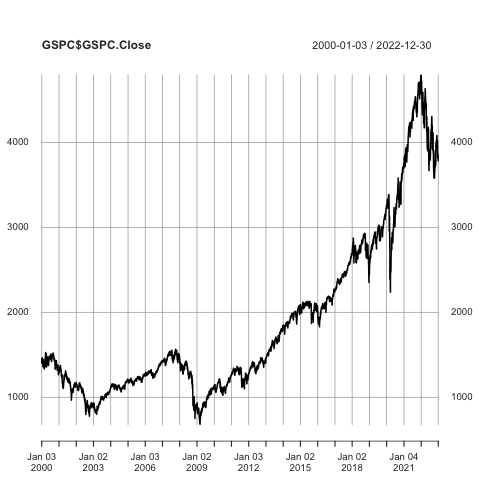
\includegraphics[width=\linewidth,height=4cm]{Figure/GSPC.png}
    \caption{S\&P 500 index}
    \label{f1}
  \end{minipage}
  \hfill
  \begin{minipage}{0.4\textwidth}
    \centering
    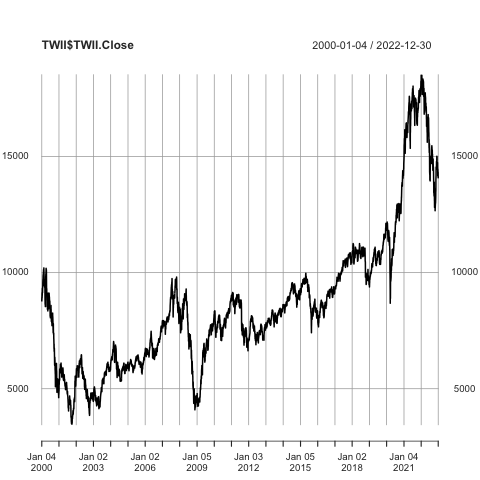
\includegraphics[width=\linewidth,height=4cm]{Figure/TWII.png}
    \caption{TAIEX}
    \label{f2}
  \end{minipage}
  \begin{minipage}{0.4\textwidth}
  \centering
    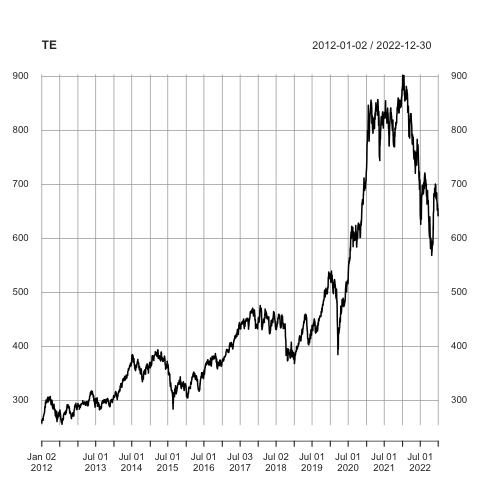
\includegraphics[width=\linewidth,height=4cm]{Figure/TE.png}
    \caption{TE}
    \label{f3}
  \end{minipage}
  \hfill
  \begin{minipage}{0.4\textwidth}
  \centering
    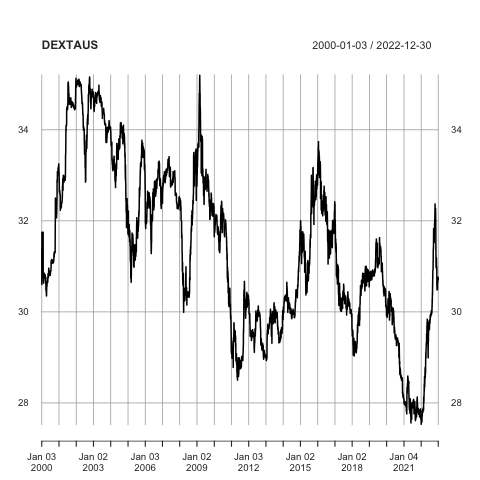
\includegraphics[width=\linewidth,height=4cm]{Figure/DEXTAUS.png}
    \caption{Nominal exchange rate}
    \label{f4}
  \end{minipage}  
\end{figure}



\section{Empirical Results}



\subsection{In-sample predictive regression results}

We now estimate the equation \ref{e1}. We first use $\Delta sp_t$ calculated from TAIEX and then use TE to calculate $\Delta sp_t$.

Table \ref{t4} provides the results.


\begin{table}
\caption{In-sample estimation}
\label{t4}
\begin{tabular}{lllll}
\textbf{Index} & \textbf{$\hat \beta$} & \textbf{SE} & \textbf{t-stat.} & \textbf{$\Pr(>|t|)$} \\
TAIEX & -1.8806e-02 & 3.1656e-03 & -5.9409 & 3.012e-09 ***  \\
TE & -1.6841e-02 & 5.2700e-03 & -3.1956 & 0.001413 **  \\
\end{tabular}
\end{table}

Somewhat unexpectedly, The negative sign of $\hat \beta$ indicates that a higher return in the Taiwan stock market is associated with an appreciation of the New Taiwan dollar. But, overall, the stock return differentials do have statistically significant predictive power.



\subsection{Out-of-sample forecasting performance}

Now, we can get the predicted values from the above models. Notice that due to our model structure, the predicted value would be $\hat r_{t+1}=\hat s_{t+1}-s_t$, but only $\hat s_{t+1}$ is of interest. Hence, we will need to "recover" the predicted values by adding the corresponding $s_t$ (One can also take exponential to recover from logarithm, but we will not do this here). However, we still use $\hat e_{t+1}=r_{t+1}-\hat r_{t+1}$ to calculate MSPE.

Table \ref{t5} and \ref{t6} provide the results.

\begin{table}
\caption{Out-of-sample prediction: TAIEX}
\label{t5}
\begin{tabular}{lll}
\textbf{h} & \textbf{$\hat r_{t+1}$} & \textbf{$\hat s_{t+1}$}  \\
1 & 3.323199e-05 &  3.421033 \\
3 & 4.897587e-05  & 3.417120 \\
5 & 2.430065e-04 & 3.421896 \\
20 & -1.151633e-04 &  3.424473  \\
\end{tabular}
\end{table}

\begin{table}
\caption{Out-of-sample prediction: TE}
\label{t6}
\begin{tabular}{lll}
\textbf{h} & \textbf{$\hat r_{t+1}$} & \textbf{$\hat s_{t+1}$}  \\
1 & 4.483858e-06 &  3.421004 \\
3 & 9.004626e-05  & 3.417161 \\
5 & 2.136861e-04 & 3.421867 \\
20 & -9.088663e-05 &  3.424497  \\
\end{tabular}
\end{table}


We will also need to calculate the mean squared prediction errors to conduct the DM hypothesis test. The result are shown in equation \ref{e4} and \ref{e5}:

\begin{align}
\label{e4}
\widehat \text{MSPE}^{\text{SRD, TAIEX}} &=\frac{1}{P}\sum (\hat e^{\text{SRD, TAIEX}}_{t+1})^2 &=5.305338e-06\\
\widehat \text{MSPE}^{\text{SRD, TE}} &=\frac{1}{P}\sum (\hat e^{\text{SRD, TE}}_{t+1})^2 &=5.221116e-06
\label{e5}
\end{align}

From equation \ref{e4} and \ref{e5}, we can see $\widehat \text{MSPE}^{\text{SRD, TE}}<\widehat \text{MSPE}^{\text{SRD, TAIEX}}$. This somewhat supports the argument we mentioned earlier that due to the importance of exports to Taiwan, focusing on the stock return differentials of the main export industry may be helpful to predict the daily exchange rates.

As for the random walk model, we first notice that if we assume the logarithm of exchange rates follows random walk, i.e., 

\begin{align}
s_{t+1}=s_t+\epsilon_{t+1}, \quad \epsilon_t\sim i.i.d(0, \sigma^2)
\end{align}

Then we have

\begin{align}
E_t(s_{t+1}-s_t)\approx E_t(r_{t+1}) =0
\end{align}

i.e., the unchanged forecasts would be the forecasts from random walk model:

\begin{align}
\hat r^{\text{RW}}_{t+1}=0
\end{align}

where $r_{t+1}=s_{t+1}-s_t$. 

The forecast error would be:

\begin{align}
\hat e^{\text{RW}}_{t+1}=(r_{t+1}-\hat r^{\text{RW}}_{t+1})^2=(r_{t+1})^2
\end{align}

Hence, the mean squared prediction error would be:

\begin{align}
\widehat \text{MSPE}^{\text{RW, TAIEX}}&=\frac{1}{P}\sum (\hat e^{\text{RW, TAIEX}}_{t+1})^2 &= 5.357038e-06\\
\widehat \text{MSPE}^{\text{RW, TE}}&=\frac{1}{P}\sum (\hat e^{\text{RW, TE}}_{t+1})^2 &= 5.357038e-06
\end{align}

Unsurprisingly, $\widehat \text{MSPE}^{\text{RW, TAIEX}}$ and $\widehat \text{MSPE}^{\text{RW, TE}}$ agree (because the calculation for MSPE of random walk model does not involve any estimation, and the difference in TAIEX and TE occurs in the predictor but not the dependent variable). Also, our regression models with the stock return differentials as predictors (either calculated from TAIEX or TE) have better performance than the random walk model, albeit this may not be statistically significant.

Finally, to test whether the improvement is statistically significant, we provide the DM statistics. To do this, we define:

\begin{align}
d_t^{\text{TAIEX}} &= (\hat e^{\text{RW}}_{t+1})^2-(\hat e^{\text{SRD, TAIEX}}_{t+1})^2\\
d_t^{\text{TE}} &= (\hat e^{\text{RW}}_{t+1})^2-(\hat e^{\text{SRD, TE}}_{t+1})^2
\end{align}

Then, regress $d_t$ on a constant $\delta$ with Newey-West HAC standard errors ($sd(\hat \delta)$). The regression model is 

\begin{align}
d_t=\delta +u_t
\end{align}

The DM statistics is $\text{DM}=\frac{\hat \delta}{sd(\hat \delta)}$

Table \ref{t7} provides the corresponding results.

\begin{table}
\caption{DM statisitics}
\label{t7}
\begin{tabular}{lllll}
\textbf{index} & \textbf{$\hat \delta$} & \textbf{$sd(\hat \delta)$} & \textbf{t-stat.} & \textbf{$\Pr(>|t|)$} \\
TAIEX & 5.1701e-08 &  2.6651e-07 & 0.194 & 0.8482 \\
TE & 1.3592e-07  & 2.4563e-07 & 0.5534 & 0.5865 \\
\end{tabular}
\end{table}

Unfortunately, in either case, we cannot reject the null hypothesis. This indicates that our regression models can not beat the simple random walk model even though we do see some mild improvement by focusing on the main export industry. 

\section{Robustness Checks}

\subsection{Estimating Using the Same Time Period for Validation}

In our study, we observed a subtle improvement when utilizing the TE data compared to the TAIEX data. However, upon closer examination, we identified a potential confounding factor: the distinct time spans covered by the two data sets. Specifically, the TAIEX data encompassed a wider time frame, beginning from 2000 and extending until 2022, while the TE data only covered the period from 2012 to 2022. Consequently, it is crucial to evaluate the influence of this temporal discrepancy to ascertain the true significance of the observed differences.

To address this concern, we conducted robustness checks using the same time period for both the TE and TAIEX data by restricting our analysis to the common time window of 2012 to 2022.

The result is presented in Table \ref{t8}.

\begin{table}
\caption{Robustness Checks: common time window}
\label{t8}
\begin{tabular}{lllll}
\textbf{Index} & \textbf{$\hat \beta$} & \textbf{SE} & \textbf{t-stat.} & \textbf{$\Pr(>|t|)$} \\
TAIEX & -1.2441e-02 & 5.7270e-03 & -2.1724 & 0.02992 *
\end{tabular}
\end{table}

The predictive power is now even weaker than that of using TE data. This supports the usefulness of using the main export industry to calculate the stock return differentials.

\subsection{Estimating Using Rolling Window}

Instead of using fixed scheme, where the in-sample observations are fixed, one can also consider the rolling window approach to obtain the one-ahead forecasts. We then use these forecasts to calculate the MSPE.

Table \ref{t9} presents the MSPE calculated by rolling approach. However, we did not see much benefits obtained from this approach.

\begin{table}
\caption{Robustness Checks: rolling window approach}
\label{t9}
\begin{tabular}{ll}
\textbf{Index} & \textbf{MSPE}\\
TAIEX & 5.31829e-06 \\
TE & 5.224172e-06
\end{tabular}
\end{table}

\section{Conclusions}

This paper explores the usefulness of stock return differentials in predicting daily exchange rate movements in Taiwan. We employed a method proposed by \cite{chen2019stock} to investigate the predictive content of stock market data for exchange rate movements. Specifically, we incorporate the stock index of main export industry, given Taiwan's export-driven economy and the significant role of exchange rates in its economic growth and competitiveness.

The regression models utilizing stock return differentials did not outperform the random walk model in a statistically significant manner, highlighting the continued challenge of accurately forecasting exchange rates.

Nonetheless, the study's focus on the main export industry in Taiwan provided some mild improvement in predictive performance. Given Taiwan's reliance on international trade and the potential undervaluation policy of its central bank, understanding the relationship between stock returns of the export industry and exchange rate movements is valuable for predicting exchange rates.




\end{spacing}

\newpage

\bibliographystyle{aea}
\bibliography{references}


\end{document}
